\documentclass{handout} 
\usepackage{handoutSetup}\usepackage{handoutShortcuts} % 
% A good follow-up handout (or exam question) would look at the augmented model in \cite{ghosDespiteUzawa}
\usepackage[noheads,nolists,nomarkers]{endfloat}
\begin{document}
\handoutHeader

\begin{verbatimwrite}{\jobname.title}
  The Ramsey/Cass-Koopmans (RCK) Model
\end{verbatimwrite}

\handoutNameMake

\newboolean{NumericalSolution}
\setboolean{NumericalSolution}{true}
% \setboolean{NumericalSolution}{false}


\renewcommand{\cite}{\citeyearpar}

Ramsey~\cite{ramseySave}, followed much later by Cass~\cite{cass:growth} and Koopmans~\cite{koopmans:growth}, formulated the canonical model of optimal growth for an economy with exogenous `labor-augmenting' technological progress.

\section{The Budget Constraint}

The economy has a perfectly competitive production sector that uses a Cobb-Douglas aggregate production function 
\begin{equation}\begin{gathered}\begin{aligned}
  % \Inc_{t} & =  \ProdFunc_{t}(\Kap,\Labor) = \Kap^{\kapShare}(\PtyLab_{t} \Labor)^{1-\kapShare}
                   \Inc & =  \ProdFunc(\Kap,\Labor) = \Kap^{\kapShare}(\PtyLab \Labor)^{1-\kapShare}
\end{aligned}\end{gathered}\end{equation}
to produce output using capital and labor.\footnote{All Roman variables are functions of time, but putting time subscripts on everything would clutter the notation, so we do it only where necessary for clarity.}  Labor hours (the same as population) increases exogenously at a constant rate\footnote{The ancient Greek philosophers captured eternal truths; therefore, Greek letters represent constants whose value never changes.}
\begin{equation}\begin{gathered}\begin{aligned}
  \dot{\Labor}/\Labor & =  \popGro
\end{aligned}\end{gathered}\end{equation}
and $\PtyLab $ is an index of labor productivity that grows at rate \opt{MarginNotes}{\marginpar{\tiny Digression on kinds of technical progress; they're all the same in a Cobb-Douglas pdn fcn.  Solow-Phelps showed: SS growth is independent of fraction
    of progress that is embodied; but speed of convergence is faster with more embodiment.}}
\begin{equation}\begin{gathered}\begin{aligned}
  \dot{\PtyLab }/\PtyLab  & =  \ptyGro. 
\end{aligned}\end{gathered}\end{equation}

Thus, technological progress allows each worker to\opt{MarginNotes}{\marginpar{\tiny Peculiar assumption; seems more natural to imagine that technology is embodied in new $K$ than in $\PtyLab \Labor$ form.  However, 60s lit showed same steady-states, and similar transitions, with embodied $K$.  Since this is simpler, we use it.}}
produce perpetually more  as time goes by with the same amount of 
physical capital.\footnote{This is the definition of `labor-augmenting' (Harrod-neutral) 
  productivity growth; with a Cobb-Douglas production function, it turns out to be essentially the same as `capital-augmenting' productivity growth, also known as Hicks-neutral, as well as output-neutral (`Solow-neutral') progress.}  The quantity $\PtyLab \Labor$ is known as the number of `efficiency 
units' of labor in the economy.

Aggregate capital accumulates according to
\begin{equation}\begin{gathered}\begin{aligned}
  \dot{\Kap} & =  \Inc - \Cons - \depr K \label{eq:Kdotlevel}.
\end{aligned}\end{gathered}\end{equation}

Lower case variables are the upper case version divided by efficiency units, i.e.
\begin{equation}\begin{gathered}\begin{aligned}
  \inc & =  \Inc/(\PtyLab \Labor)  \\
       & =  \Kap^{\kapShare}(\PtyLab \Labor)^{1-\kapShare}/(\PtyLab \Labor)  \\
       & =  (\Kap/\PtyLab \Labor)^{\kapShare}
  \\   & =  \kap^{\kapShare}    .
\end{aligned}\end{gathered}\end{equation}

Note that 
\begin{equation}\begin{gathered}\begin{aligned}
  \dot{\kap} \equiv       \left(\frac{d\kap}{dt}\right) & =  \left(\frac{\dot{\Kap}\PtyLab \Labor - K(\dot{\PtyLab }L + \PtyLab \dot{\Labor})}{(\PtyLab \Labor)^{2}}\right) 
  \\   & =  \dot{\Kap}/\PtyLab \Labor - k(\dot{\PtyLab }/{\PtyLab } + \dot{\Labor}/\Labor)
  \\          & =  \dot{\Kap}/\PtyLab \Labor - (\ptyGro +\popGro)k
\end{aligned}\end{gathered}\end{equation}
which means that \eqref{eq:Kdotlevel} can be divided by $\PtyLab \Labor$ and becomes
\begin{equation}\begin{gathered}\begin{aligned}
  \dot{\Kap}/\PtyLab \Labor & =  \inc - \cons - \depr \kap  \\
  \dot{\kap}+(\ptyGro +\popGro)k & =  \prodFunc(\kap) - \cons - \depr \kap  \\
  \dot{\kap} & =  \prodFunc(\kap) - \cons - (\ptyGro +\popGro+\depr) \kap \label{eq:kdot}.
\end{aligned}\end{gathered}\end{equation}

A steady-state will be a point where $\dot{\kap} = 0$.

Equation~\eqref{eq:kdot}  yields a first candidate for an optimal
steady-state of the growth model: It seems reasonable to argue that the best
possible steady-state is the one that maximizes $\cons$.  This is the
``golden rule'' optimality condition of
Phelps~\cite{phelps:golden}, an article well worth reading; this is
one of the chief contributions for which Phelps won the Nobel prize.

\section{The Social Planner's Problem}

Now suppose that there is a social planner whose goal is to maximize the discounted
sum of CRRA utility from per-capita consumption:
\begin{equation}
  \max \int_{0}^{\infty} \left(\frac{(\Cons/\Labor)^{1-\CRRA}}{1-\CRRA}\right) e^{-\timeRate  t} \label{eq:maxprob}.  
\end{equation}

But $\Cons/\Labor = \PtyLab (\Cons/\PtyLab \Labor)= \PtyLab c$.  Recall that for a variable growing at rate $\ptyGro$,
\begin{equation}\begin{gathered}\begin{aligned}
  \PtyLab _{t} & =  \PtyLab _{0}e^{\ptyGro t}
\end{aligned}\end{gathered}\end{equation}
so if the economy started off in period 0 with productivity $\PtyLab_{0}$, by date $t$ we can rewrite
\begin{equation}\begin{gathered}\begin{aligned}
  \Cons/\Labor & =  c\PtyLab   \\
               & =  c\PtyLab _{0}e^{\ptyGro t}. \label{eq:cRat}
\end{aligned}\end{gathered}\end{equation}

Using \eqref{eq:cRat} and the other results above, we can rewrite the social planner's objective function as
\begin{equation}\begin{gathered}\begin{aligned}
  \int_{0}^{\infty} \left(\frac{(\PtyLab c)^{1-\CRRA}}{1-\CRRA}\right) e^{-\timeRate  t} & =  
                                                                                               \PtyLab _{0}^{1-\CRRA}\int_{0}^{\infty} \left(\frac{\cons^{1-\CRRA}}{1-\CRRA}\right) e^{-\timeRate  t}e^{(1-\CRRA)\ptyGro  t} 
  \\ & =  \PtyLab _{0}^{1-\CRRA}\int_{0}^{\infty} \util(c) e^{\left((1-\CRRA)\ptyGro -\timeRate \right) t}
           .
           \label{eq:maxprobmod}
\end{aligned}\end{gathered}\end{equation}

Thus, defining $\nu = \timeRate  - (1-\CRRA) \ptyGro$ and normalizing the initial
level of productivity to $\PtyLab _{0}=1$, the complete optimization problem
can be formulated as
\begin{equation}
  \max \int_{0}^{\infty} \util(c) e^{-\nu  t}
\end{equation}
subject to
\begin{equation}
  \dot{\kap} = \kap^{\kapShare}-\cons-(\popGro+\ptyGro+\depr)k,
\end{equation}
which has a discounted Hamiltonian representation
\begin{equation}
  \Ham(\kap,c,\lambda) = \util(c) + (\kap^{\kapShare} - \cons - (\popGro+\ptyGro+\depr)\kap)\lambda.
\end{equation}

The first \href{https://en.wikipedia.org/wiki/Hamiltonian_(control_theory)}{discounted Hamiltonian optimization condition} requires $\partial 
\Ham/\partial \cons = 0$:
\begin{equation}\begin{gathered}\begin{aligned}
  c^{-\CRRA} & =  \lambda  \label{eq:H1A} \\
  -\CRRA c^{-\CRRA-1}\dot{\cons} & =  \dot{\lambda} 
                                       .
\end{aligned}\end{gathered}\end{equation}

The second discounted Hamiltonian optimization condition requires:
\begin{equation}\begin{gathered}\begin{aligned}
  \dot{\lambda} & =  \nu\lambda - \partial \Ham/\partial \kap  \\
                & =  \nu\lambda - \lambda (\prodFunc^{\prime}(\kap) - (\popGro+\ptyGro+\depr))  \\
  \dot{\lambda}/{\lambda} & =  (\nu+(\popGro+\ptyGro+\depr)-\prodFunc^{\prime}(\kap))
  \\  \left(\frac{-\CRRA c^{-\CRRA-1}\dot{\cons}}{\cons^{-\CRRA}}\right) & =  (\nu+(\popGro+\ptyGro+\depr)-\prodFunc^{\prime}(\kap))
  \\  \CRRA \dot{\cons}/\cons & =  (\prodFunc^{\prime}(\kap)-\nu-(\popGro+\ptyGro+\depr))
  \\  \dot{\cons}/\cons  & =  \CRRA^{-1}(\underbrace{\prodFunc^{\prime}(\kap)-(\popGro+\ptyGro+\depr)}_{\mbox{$\equiv \acute{r}$}}-\nu)
\end{aligned}\end{gathered}\end{equation}
where the definition of $\acute{r}$ is motivated by thinking of 
$\prodFunc^{\prime}(\kap)-(\popGro+\ptyGro+\depr)$ as the interest rate net of depreciation and
dilution.  

This is called the ``modified golden rule'' (or sometimes the 
``Keynes-Ramsey rule'' because it was originally derived by 
Ramsey with an explanation attributed to Keynes).  

Thus, we end up with an Euler equation for consumption growth that is
just like \href{https://www.econ2.jhu.edu/people/ccarroll/public/LectureNotes/Consumption/PerfForesightCRRA/#EulerCGroFac}{the Euler equation in the perfect foresight partial equilibrium consumption model}, except that now the relevant interest rate can vary over
time as $\prodFunc^{\prime}(\kap)$ varies.

Substituting in the modified time preference rate gives
\begin{equation}\begin{gathered}\begin{aligned}
  \dot{\cons}/\cons  & =  \CRRA^{-1}(\prodFunc^{\prime}(\kap)-(\popGro+\depr+\ptyGro)-\timeRate  +(1- \CRRA) \ptyGro)
  \\   & =  \CRRA^{-1}(\prodFunc^{\prime}(\kap)-(\popGro+\depr)-\timeRate  - \CRRA \ptyGro), \label{eq:cdotOc}
\end{aligned}\end{gathered}\end{equation}
and finally note that defining per capita consumption $\chi = \Cons/\Labor$
so that $\cons = \chi \PtyLab ^{-1}$, 
\begin{equation}\begin{gathered}\begin{aligned}
  \label{eq:chiDotOchi}
  \dot{\cons} & =  \dot{\biggl(\chi \PtyLab ^{-1}\biggr)} =  \dot{\chi}\PtyLab ^{-1}-(\chi \PtyLab ^{-1})\dot{\PtyLab }/\PtyLab 
  \\ \dot{\cons}/\cons & =  \dot{\biggl(\chi \PtyLab ^{-1}\biggr)}/(\chi \PtyLab^{-1}) =  \dot{\chi}/\chi - \ptyGro 
\end{aligned}\end{gathered}\end{equation}
and since \eqref{eq:cdotOc} can be written
\begin{equation}\begin{gathered}\begin{aligned}
  \dot{\cons}/\cons  & =  \CRRA^{-1}(\prodFunc^{\prime}(\kap)-(\popGro+\depr)-\timeRate ) - \ptyGro,
\end{aligned}\end{gathered}\end{equation}
we have
\begin{equation}\begin{gathered}\begin{aligned}
  \dot{\chi}/\chi & =  \CRRA^{-1}(\prodFunc^{\prime}(\kap)-(\popGro+\depr)-\timeRate )
\end{aligned}\end{gathered}\end{equation}
so the formula for per capita consumption growth (as a function of
$\kap$) is identical to the model with no growth (equation
\eqref{eq:cdotOc} with $\ptyGro=0$).  Any important differences between
the no-growth model and the model with growth therefore must come
through the channel of differences in $\kap$.


\section{The Steady State}

The assumption of labor augmenting technological progress was made 
because it implies that in steady-state, per-capita consumption, income,
and capital all grow at rate $\ptyGro$.\footnote{See~\cite{ghosDespiteUzawa} for a discussion of the realism of this requirement.}

$\dot{\cons}/\cons = 0$ implies that at the steady-state value of $\check{\kap}$,
\begin{equation}\begin{gathered}\begin{aligned}
  \prodFunc^{\prime}(\check{\kap}) & =  \timeRate +\popGro+\depr+\CRRA \ptyGro  \\
  \kapShare \check{\kap}^{\kapShare-1} & =  \timeRate +\popGro+\depr+\CRRA \ptyGro  \\
  \check{\kap} & =  \left(\frac{\timeRate +\popGro+\depr+\CRRA \ptyGro}{\kapShare}\right)^{\frac{1}{\kapShare-1}}
  \\      \check{\kap} & =  \left(\frac{\kapShare}{\timeRate +\popGro+\depr+\CRRA \ptyGro}\right)^{\frac{1}{1-\kapShare}}   
\end{aligned}\end{gathered}\end{equation}

Thus, the steady-state $\kap$ will be higher if capital 
is more productive ($\kapShare$ is higher), and will be lower if 
consumers are more impatient, population growth is faster, 
depreciation is greater, or technological progress occurs more rapidly.

\section{A Phase Diagram}

While the RCK model has an analytical solution for its steady-state,
it does not have an analytical solution for the transition to the 
steady-state.  The usual method for analyzing
models of this kind is a \href{https://en.wikipedia.org/wiki/Phase_diagram}{phase diagram} in $\cons$ and $\kap$.  
The first step in constructing the phase diagram is to take the differential
equations that describe the system and find the points where they are 
zero.  Thus, from \eqref{eq:kdot} we have that $\dot{\kap}=0$ implies
\begin{equation}\begin{gathered}\begin{aligned}
  \cons & =  \prodFunc(\kap) - (\ptyGro +\popGro+\depr) \kap \label{eq:kdotEq0}
\end{aligned}\end{gathered}\end{equation}
and we have already solved for the (constant) $\check{\kap}$ that characterizes
the $\dot{\cons}/\cons=0$ locus.  These can be combined to generate the borders between
the phases in the phase diagram, as illustrated in figure~\ref{fig:RamseySSPlot}.
\opt{MarginNotes}{\marginpar{\tiny 
    There's an inconsistency between the programs, in the Ramsey directory,
    that generated these figures and the notes here: the programs assume
    $\util(\cons \Labor)/\Labor$ and here we assume $\util(c)$.
  }}
\begin{figure}
  \caption{$\dot{\cons}/\cons =0 $ and $\dot{\kap}=0$ Loci}\label{fig:RamseySSPlot}
  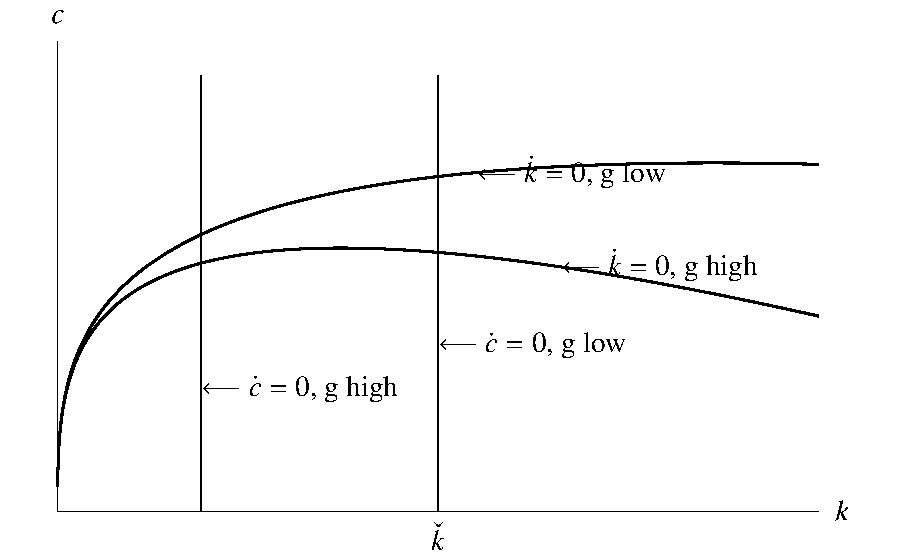
\includegraphics[width=6in]{../Figures/RamseySSPlot}
\end{figure}

\section{Transition}

Actually, as stated so far, the solution to the problem is very simple: The
consumer should spend an infinite amount in every period.  This solution is 
not ruled out by anything we have yet assumed (except possibly the fact that
once $\kap$ becomes negative the production function is undefined).  

Obviously, this is not the solution we are looking for.  What is missing is
that we have not imposed anything corresponding to the intertemporal 
budget constraint.  In this context, the IBC takes the form of a ``transversality
condition,'' 
\begin{equation}\begin{gathered}\begin{aligned}
  \label{eq:tvc}
  \lim_{t \rightarrow \infty} \lambda_{t} e^{(\ptyGro +\popGro) t - \int_{0}^{t} r_{\tau} d\tau }k_{t} & =  0.
\end{aligned}\end{gathered}\end{equation}

The intuitive purpose of this unintuitive equation is basically to prevent
the capital stock from becoming negative or infinity as time goes by.  
Obviously a capital stock that was negative for the entire future could not 
satisfy the equation.  And a capital stock that is too large will have 
an arbitrarily small interest rate, which will result in the LHS of the 
TVC being a positive number, again failing to satisfy the TVC.

Figure~\ref{fig:RamseySaddlePlot} shows three paths for $\cons$ and $\kap$
that satisfy \eqref{eq:cdotOc} and \eqref{eq:kdot}.  The topmost path,
however, is clearly on a trajectory toward zero then negative
$\kap$, while the bottommost path is heading toward an infinite
$\kap$.  Only the middle path, labelled the ``saddle path,'' satisfies
both \eqref{eq:cdotOc} and \eqref{eq:kdot} as well as the TVC
\eqref{eq:tvc}.

\begin{figure}
  \caption{Transition to the Steady State}\label{fig:RamseySaddlePlot}
  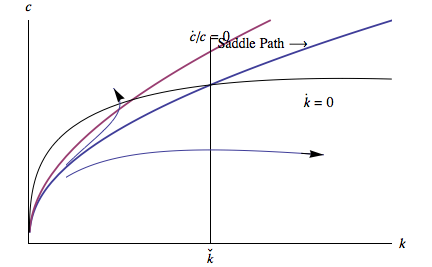
\includegraphics[width=6in]{../Figures/RamseySaddlePlot}
\end{figure}

\section{Interactive Notebooks}

An explicit numerical solution to the Ramsey problem, with a description of a solution method and its
mathematical/computational underpinnings, is available \href{https://github.com/llorracc/Jupyter/blob/master/notebooks/RamseyCassKoopmans.ipynb}{here}.



\input handoutBibMake.tex

% For some reason the attempt to compile the code below creates an unrecoverable error in dvi mode 
\ifdvi
\setboolean{NumericalSolution}{false}
\fi

\ifthenelse{\boolean{NumericalSolution}}{
  \pagebreak\centerline{\bf \Large Appendix: Numerical Solution} \medskip\medskip

  The RCK model does not have an analytical solution, which means that
  numerical methods must be used to find out the model's quantitative
  implications for transition paths.  

  The method of solution of these kinds of models is not important for
  the purposes of first year graduate macroeconomics; this appendix 
  has been written as a reference for more advanced students who might
  be beginning their research on growth models.

  The most straightforward method of numerical solution for perfect foresight
  models of this kind is called the
  `time elimination' method.  It starts from the fact that
  \begin{equation}\begin{gathered}\begin{aligned}
    \left(\frac{d\cons/dt}{d\kap/dt}\right) &=  d\cons/d\kap.
  \end{aligned}\end{gathered}\end{equation}

  Note from \eqref{eq:cdotOc} that we can write
  \begin{equation}\begin{gathered}\begin{aligned}
    \dot{\cons} & =   \CRRA^{-1}(\prodFunc^{\prime}(\kap)-\timeRate -(\popGro+\depr)-\CRRA \ptyGro)\cons \label{eq:cdot},
  \end{aligned}\end{gathered}\end{equation}
  so we can obtain 
  \begin{equation}\begin{gathered}\begin{aligned}
    d\cons/d\kap & =  \left(\frac{(\kapShare \kap^{\kapShare-1}-\timeRate -(\popGro+\depr)-\CRRA \ptyGro)\cons}
                       {\CRRA(\kap^{\kapShare} - \cons - (\ptyGro +\popGro+\depr) \kap)}\right)
  \end{aligned}\end{gathered}\end{equation}
  which is a differential equation with no analytical solution.  Many numerical math packages can solve differential equations numerically, yielding a numerical version of the $\cFunc(\kap)$ function.

  There is one problem, however, which is that at the steady-state values of $\cons$ and $\kap$ both numerator and denominator of this equation are zero.  The alternative is to solve the differential equation twice: Once for a domain extending from $\kap=0$ to $\check{\kap}-\epsilon$, yielding $\cFunc_{-}(\kap)$, and once for a domain from $\check{\kap}+\epsilon$ to some large value of $\kap$, yielding $\cFunc_{+}(\kap)$. The true consumption policy function can then be approximated by interpolating between the upper endpoint of $\cFunc_{-}(\kap)$ and the lower endpoint of $\cFunc_{+}(\kap)$.

  For further details of he numerical solution of this model, see \href{https://github.com/llorracc/Jupyter/notebooks/RamseyCassKoopmans.ipynb}{this Jupyter notebook}, or clone the repo and, in the cloned directory, run the corresponding python program: \texttt{ipython RamseyCassKoopmans.py}.


}{}

\end{document}
